\documentclass[11pt]{article}
\usepackage[includeheadfoot, top=1.0in, bottom=1.0in, hmargin=1.0in]{geometry}
\usepackage[utf8]{inputenc}
\usepackage{fancyhdr}
\pagestyle{fancy}
\usepackage{setspace}
\usepackage{tabularx}
\usepackage{xcolor}
\usepackage{cancel}
\usepackage{amsmath,amsfonts}
\usepackage{graphicx}
\usepackage{siunitx}
\usepackage{amssymb}

\usepackage[hyphens]{url}
\usepackage{hyperref}

\lhead{Astronomy Lab II}
\rhead{Spring 2022}
\lfoot{Mead}
\rfoot{Mon 6-9pm}
\cfoot{\thepage}

\begin{document}

\begin{center}
\huge{Lab 2: Exploring the Multiwavelength Universe}\\ \medskip \Large{January 31, 2022}
\end{center}

%%%%%%%%%%%%%%%%%%%%%%% INTRO %%%%%%%%%%%%%%%%%%%%%%%
\section{Introduction: Let There Be Light}
At its core, observational astronomy is the art of collecting light. All luminous matter in the Universe -- from the tiniest grain of dust to the most massive cluster of galaxies -- emits light in some shape or form. As astronomers, it's our job to capture and interpret this ever-present light.

\medskip \noindent
While some light can be effectively processed by the naked eye (we call this ``visible'' or ``optical'' light), the majority of light in the Universe is imperceptible to humans. Electromagnetic radiation (just a fancy, science-y term for light) spans a broad \emph{spectrum} of flavors, from low-frequency radio waves to high-energy gamma rays (see Figure \ref{fig:spectrum}). Astronomical objects emit electromagnetic radiation across the entire spectrum; therefore, in order to fully understand the Universe, we must be able to observe all varieties of light. While we as humans cannot \emph{see} microwaves or radio waves or X-rays, we are more than capable of building special detectors that can. Collectively, we refer to these detectors as ``telescopes.''

\medskip \noindent
In this lab, you will learn about the variety of light comprising the ``electromagnetic spectrum.'' You will explore a range of astronomical objects producing light in all regions of the spectrum, thus demonstrating the need for a wide array of specialized telescopes. After completing this lab, you should have a deeper understanding of the nature of light, of what it means to ``observe'' the Universe, and of the utility of telescopes. These concepts form the foundations of modern astronomy. 

%%%%%%%%%%%%%%%%%%%%%%% LIGHT %%%%%%%%%%%%%%%%%%%%%%%
\section{The Anatomy of a Light Wave}
Light can be thought of as either a \emph{wave} (often referred to as an ``electromagnetic'' wave) or as a \emph{particle} (called a ``photon''). While both descriptions of light are perfectly valid, we'll primarily be focusing on the wave nature of light in this lab. When physicists refer to ``waves,'' they're referring to steady, propagating wiggles (or, in technical terms, ``oscillations''), like those illustrated in Figure \ref{fig:lightwaves}. These waves are comprised of a series of alternating \emph{peaks} (high points) and \emph{troughs} (low points); we can therefore characterize a wave by measuring its \emph{amplitude} (half the vertical distance from the bottom of a trough to the top of a peak) and its \textbf{\emph{wavelength}} (the horizontal distance from peak to peak or from trough to trough). For a light wave, the amplitude tells us how bright (or \emph{intense}) the light is. Meanwhile, the wavelength controls the ``identity'' of a light wave -- the wavelength dictates what color the light will be, how much energy is carried by the light, how deeply the light can penetrate into matter, and more. The wavelength is the key property that we'll be exploring in today's lab.

\medskip \noindent
Figure \ref{fig:lightwaves} shows only the wavelength range of ``visible'' light -- the light that we, as humans, can see with our naked eyes. Importantly, however, light can exist at wavelengths far longer and far shorter than the visible range, filling out the entire \emph{\textbf{electromagnetic (EM) spectrum}} (Figure \ref{fig:spectrum}). At the longest wavelengths, we have \emph{radio waves}; as we decrease the wavelength, we move through \emph{microwaves}, \emph{infrared light}, \emph{visible light}, \emph{ultraviolet light}, \emph{X-rays}, and \emph{gamma rays}. The wide variety of light that shines throughout the Universe makes observational astronomy an extremely rich field of study. 

\begin{figure}[t!]
    \centering
    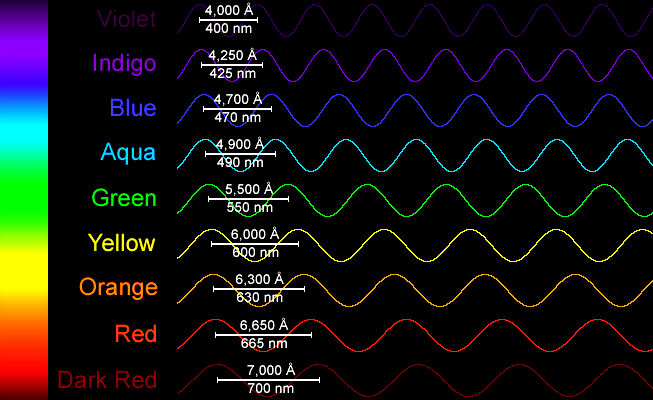
\includegraphics[width=0.8\textwidth]{Images/light waves.jpg}
    \caption{A collection of light waves with varying \emph{wavelengths}. The wavelengths are reported both in units of nanometers (nm, $10^{-9}$ meters) and in units of angstroms (\AA, $10^{-10}$ meters).}
    \label{fig:lightwaves}
\end{figure}

\begin{figure}
    \centering
    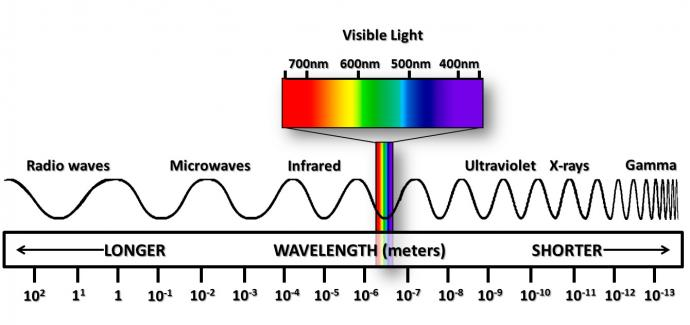
\includegraphics[width=0.8\textwidth]{Images/EM spectrum.jpg}
    \caption{The electromagnetic spectrum: the broad assortment of light that permeates the Universe.}
    \label{fig:spectrum}
\end{figure}
\medskip
\noindent
Let's think a little deeper about the electromagnetic spectrum. \textbf{Record your responses in your lab write-up}.
\begin{enumerate}
    \item Note the huge range of wavelengths covered by the electromagnetic spectrum (Figure \ref{fig:spectrum}). By how many orders of magnitude is the wavelength of a long radio wave (around $10^2$ m) greater than the wavelength of a hard gamma ray (around $10^{-13}$ m)? 
    
    \item The electromagnetic spectrum is not just relevant in astronomy -- we experience almost all wavelengths of the spectrum in our daily lives. For each region of the EM spectrum (radio, microwave, IR, visible, UV, X-ray, gamma), list one or two sources of that type of light that we may find on Earth. (\textit{Hint}: this website has some fun examples: \url{https://imagine.gsfc.nasa.gov/science/toolbox/emspectrum1.html})
    
    \item The average human body cell is 100 $\mu m$ in diameter. Compare this to the typical wavelength of a radio wave and to the typical wavelength of a gamma ray. Why do you think gamma rays are harmful to humans but radio waves are not?
    
    \item At roughly what wavelength do you think the Sun emits most of its light? (\textit{Hint}: human eyes evolved to detect sunlight)
    
    \item Navigate to \url{https://javalab.org/en/electromagnetic_waves_en/}. In the applet window, you can click and drag the mouse up and down to explore different regions of the electromagnetic spectrum.
    \begin{enumerate}
        \item As you drag the burgundy arrow from the top of the spectrum (the radio range) to the bottom of the spectrum (the X-ray range), describe qualitatively what happens to the propagating wave.
        
        \item When the burgundy arrow is near the top of the spectrum, the wave appears stationary and flat. Why is this the case?
    \end{enumerate}
    
    \item Different wavelengths of light have different \emph{optical properties}, meaning that they behave differently when sent through a prism or lens or when bounced off a mirror. This fact forms the basis of the extremely important technique of \textbf{\emph{spectroscopy}}, which we will explore at length in the next lab. For now, navigate to \url{https://javalab.org/en/electromagnetic_waves_around_of_visible_rays_en/}. In the applet window, you can click and drag the mouse up and down to vary the wavelength of light passing through the prism.
    \begin{enumerate}
        \item Light is ``bent'' as it travels through a prism. As you vary the wavelength from long wavelengths to short wavelengths, how does the degree of bending vary? Are shorter wavelengths bent more than longer wavelengths, or vice versa?
        
        \item This simulation only shows a \emph{single} wavelength of light passing through the prism at any given time. If we instead sent ``white light'' (an equal mixture of all wavelengths) through the prism, what do you expect the light pattern emerging from the prism to look like? 
        
        \item If we were instead to shine \emph{starlight} through the prism, what could the resulting light pattern tell us about the star? (give your best guess -- we'll look at this in more detail next week)
        
    \end{enumerate}
\end{enumerate}

%%%%%%%%%%%%%%%%%%%%%%% MULTIWAVELENGTH UNIVERSE %%%%%%%%%%%%%%%%%%%%%%%
\section{The Multiwavelength Universe}
The night sky shines in all wavelengths of the electromagnetic spectrum. All ordinary matter -- including that which makes up tiny dust grains, planets, stars, galaxies, etc. -- interacts with or produces light, filling the Universe with a whole zoo of different light waves. In these next few sections, we'll explore our ``Multiwavelength Universe'' in a little more depth.

\medskip \noindent
First, go to this website: \url{https://www.nao.ac.jp/study/multiwave/en/}; we'll be using this site for the next few sections of this lab. Once the site loads, click the ``start'' button in the middle of the screen. The landing page shows the electromagnetic spectrum at the bottom of the screen, with each region labeled. Clicking on any of these labels will show you an image of the Antennae Galaxies composed of light from that particular region of the spectrum (with the exception of gamma rays, for which an image of the Antennae Galaxies is not shown). Moreover, once you've clicked on a specific wavelength range, you can scroll up or down (or use the dots on the right side of the screen) to learn more about the astronomical objects and phenomena that emit this light.

\begin{enumerate}
    %\setcounter{enumi}{6}
    \item For each region of the electromagnetic spectrum, briefly describe what we can learn about the Antennae Galaxies by observing in this wavelength range. Additionally, briefly describe two astrophysical phenomena that emit this type of light. \textbf{Record these responses in your lab write-up}.
\end{enumerate}

%%%%%%%%%%%%%%%%%%%%%%% TELESCOPES %%%%%%%%%%%%%%%%%%%%%%%
\section{Why do we need so many telescopes?}

No single telescope can observe the entire electromagnetic spectrum -- if we wish to obtain consistently high-quality images of the Universe at multiple wavelengths, we need to design special detectors that are fine-tuned to receive light within relatively narrow wavelength ranges. For instance, radio telescopes typically have extremely large receivers in order to accommodate for the long wavelengths of radio light -- but, if we were to try to observe the tiny wavelengths of X-rays or gamma rays with a radio telescope, we'd barely register a detection. Similarly, if we tried to observe visible light with the narrow aperture of an X-ray telescope, we'd get a very fuzzy, saturated image. Telescope design is as much an art as it is a science. 

\begin{figure}
    \centering
    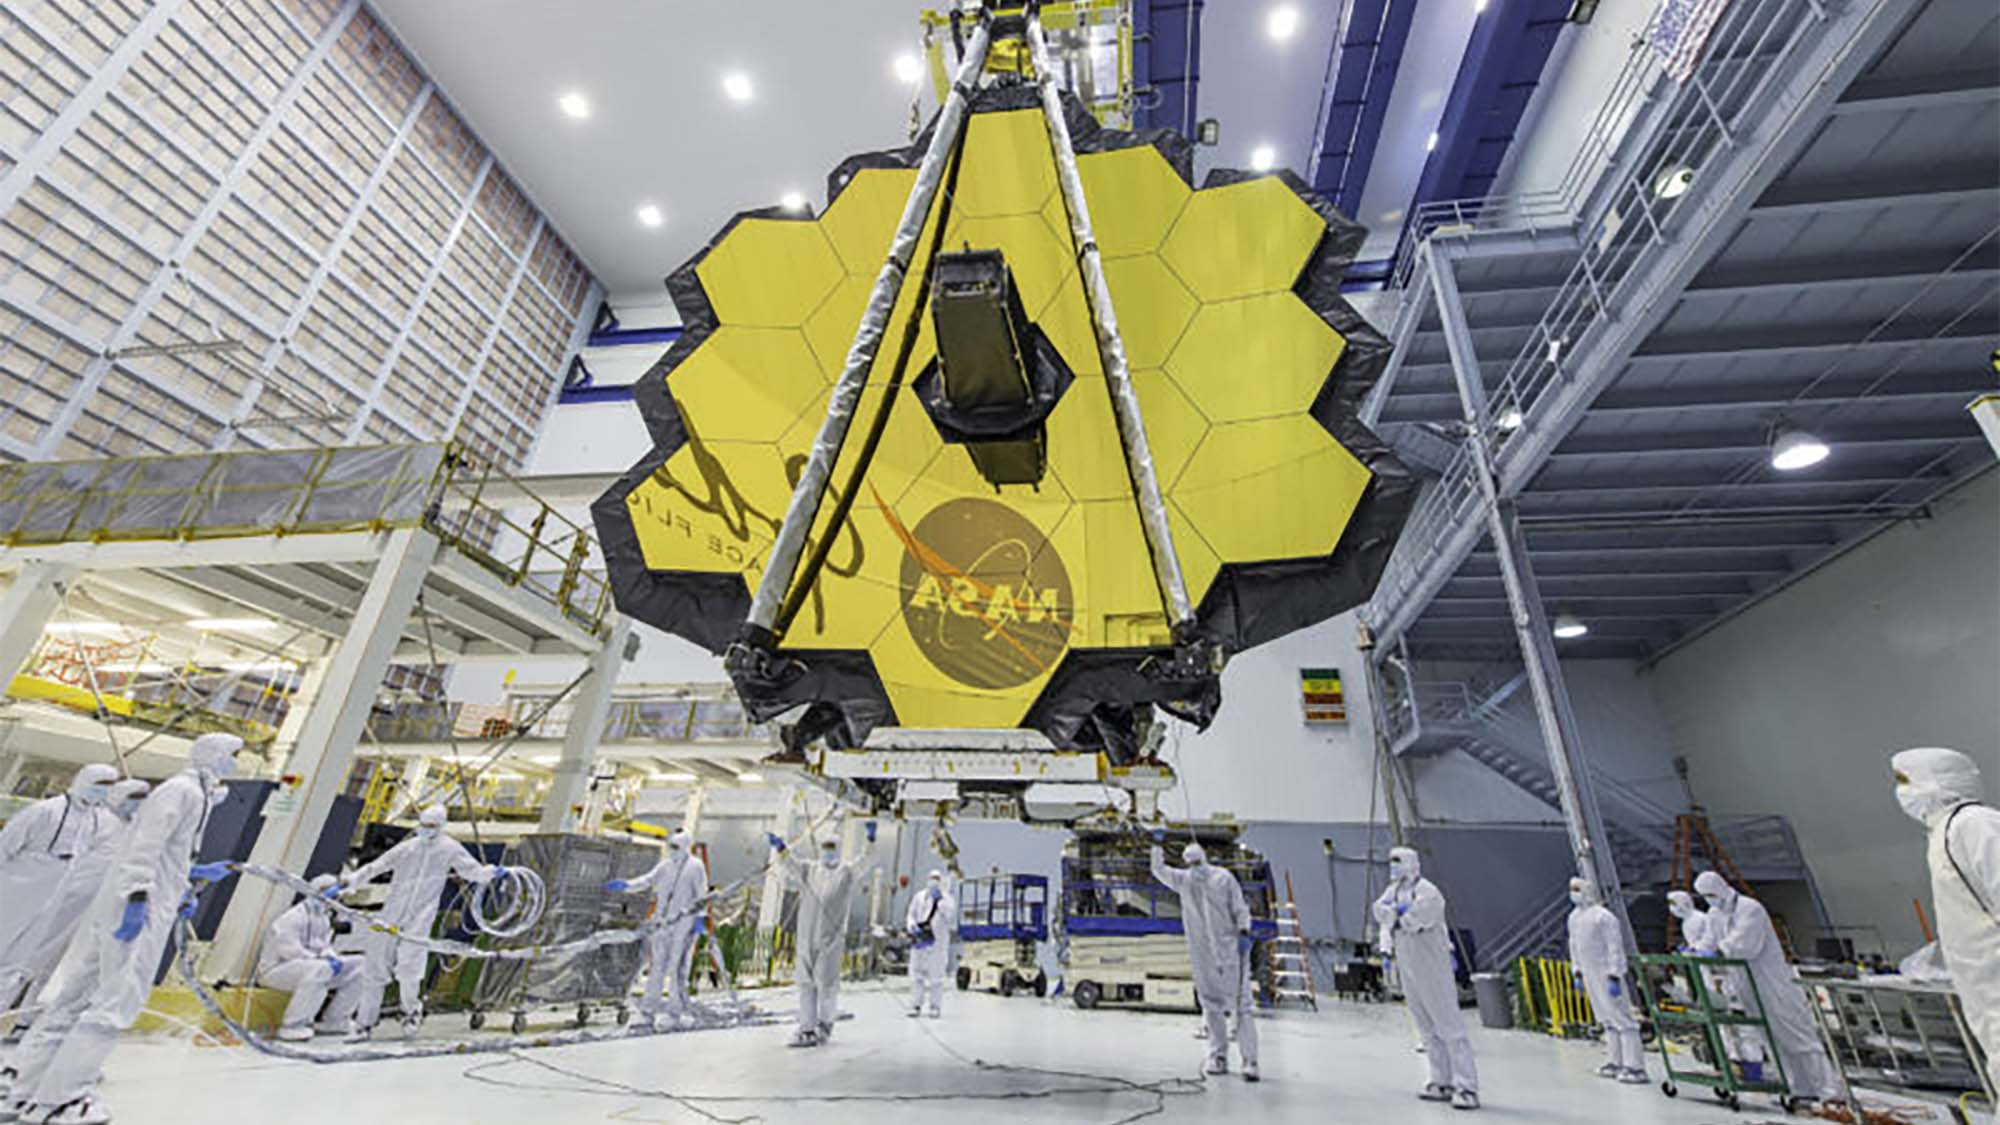
\includegraphics[width=0.6\textwidth]{Images/jwst.jpg}
    \caption{The James Webb Space Telescope (JWST) in all its glory.}
    \label{fig:jwst}
\end{figure}

\medskip \noindent
Let's take a closer look at a few telescopes. Navigate back to \url{https://www.nao.ac.jp/study/multiwave/en/}. Now, click on the tab at the bottom of the screen that says ``Wavelength Guide'' -- this'll bring up a list of telescopes organized by wavelength range. Use this page (as well as the ``Wavelengths and Targets'' tab, located at the bottom of the screen) to answer the following questions. \textbf{Record your responses in your lab write-up}.
\begin{enumerate}
    %\setcounter{enumi}{7}
    \item Just over a month ago, the brand new \textbf{James Webb Space Telescope} (JWST, see Figure \ref{fig:jwst}) was launched into space. Find JWST on the ``Wavelengths and Telescopes'' chart. Which regions of the electromagnetic spectrum is JWST tuned to detect? What type of light will JWST primarily be observing? Many news outlets have stated that JWST will ``replace'' the Hubble Space Telescope. Looking at the ``Wavelengths and Telescopes'' chart, explain why this statement is not fully accurate. What telescope would it make more sense to label as the ``predecessor'' to JWST? Take a quick look at this JWST fact sheet: \url{https://jwst.nasa.gov/content/webbLaunch/assets/documents/WebbFactSheet.pdf}. Briefly describe two science cases that JWST will be focusing on.
    
    \item The Atacama Large Millimeter/submillimeter Array -- or \emph{ALMA} -- is an array of telescopes in Chile that has been revolutionary for the study of planet formation and the study of black hole structure. Locate ALMA on the ``Wavelengths and Telescopes'' page. In which region of the electromagnetic spectrum does ALMA observe? List one type of astronomical object that ALMA can see well and very briefly describe this object. Recently, the field of ``submillimeter'' astronomy has received increased attention for its ability to probe star formation and cosmology -- why do you think this field is called ``submillimeter'' astronomy?
    
    \item You -- an early career astronomer -- have decided that X-ray astronomy will be your specialty. Naturally, you start writing up some observing proposals for a few telescopes. Which telescopes should you submit your proposals to? What are two types of astronomical objects that you could study with these telescopes? (briefly describe these objects)     
    \item You've heard some cool things about hot stars (pun intended). In what region of the electromagnetic spectrum do high-mass, high-temperature stars emit most of their light? Which telescopes would be best suited for observing these stars?  
    
    \item (\textbf{Bonus question}: complete this question if you have some extra time)  Choose at least one upcoming telescope or observatory from the list below and read a little bit about these telescopes. For each telescope, answer: What region(s) of the EM spectrum is this instrument specialized for? What's one science case that this instrument will address? How will this telescope improve on its predecessors?
    \begin{itemize}
        \item \underline{Vera C. Rubin Observatory}: 1) \url{https://www.lsst.org/content/rubin-observatory-general-public-faqs}; \, \, 2) \url{https://www.lsst.org/science}; \, \, 3) \url{https://www.lsst.org/about/fact-sheets}
        
        \item \underline{Nancy Grace Roman Space Telescope}: 1) \url{https://roman.gsfc.nasa.gov/faq.html}; \, \, 2) \url{https://roman.gsfc.nasa.gov/images/stsci/roman-capabilities-stars.pdf}; \, \, 3) \url{https://roman.gsfc.nasa.gov/images/stsci/roman-capabilities-galaxies.pdf}
        
        \item \underline{Square Kilometer Array}: 1) \url{https://www.skatelescope.org/the-ska-project/}; \, \, 2) \url{https://www.skatelescope.org/ska-prospectus/}; \, \, 3) \url{https://www.skatelescope.org/science/}
        
        \item \underline{Euclid}: 1) \url{https://sci.esa.int/web/euclid/-/summary}; \, \, 2) \url{https://sci.esa.int/web/euclid/-/fact-sheet}
    \end{itemize}
    
\end{enumerate}

%%%%%%%%%%%%%%%%%%%%%%% ATMOSPHERE %%%%%%%%%%%%%%%%%%%%%%%
\section{The Earth's atmosphere: Astronomy's greatest enemy}

Light propagates perfectly fine through vacuum (the complete absence of matter), but as soon as we introduce matter -- like the gas in the Earth's atmosphere -- we run into trouble. As light passes through our atmosphere, turbulent gas scatters and deflects this light, affecting the clarity of ground-based telescope observations (in astronomy jargon, we say that the atmosphere affects the \emph{``seeing''} of our telescopes). Moreover, certain molecules in our atmosphere -- like water, carbon dioxide, and ozone -- can \emph{absorb} incoming light, completely preventing some wavelengths from reaching the ground. So, while the Earth's atmosphere is fantastic for life on Earth, it's disastrous for ground-based astronomy.

\medskip \noindent
Let's explore the effects of the Earth's atmosphere in a bit more depth. First, navigate back to \url{https://www.nao.ac.jp/study/multiwave/en/}. Go back to the ``Wavelength Guide'' page (located at the bottom of the screen), and now click on the ``Wavelength and Atmospheric Penetration'' tab. This page should display a graphic illustrating how far different wavelengths of light can travel through our atmosphere. Using this diagram, answer the following questions. \textbf{Record your responses in your lab write-up}.
\begin{enumerate}
    %\setcounter{enumi}{12}
    \item In which wavelength ranges can light reach the surface of the Earth (i.e., an altitude of 0 km)? Referring back to the ``Wavelengths and Telescopes'' tab, what are some \emph{ground-based} telescopes that observe in these wavelength ranges? Where are these telescopes located? (\textit{Hint}: you can click on the telescope name to find the location)
    
    \item Which wavelengths are affected the most by the atmosphere? Referring back to the ``Wavelengths and Telescopes'' tab, what are some telescopes that observe at these wavelengths? Where are these telescopes located?
    
    \item Many ground-based telescopes, like the Subaru Telescope and the Keck Observatory, are built on the summits of very tall mountains. Why is the top of a mountain an optimal location for a telescope? (\textit{Hint}: think about the air quality on top of a mountain vs. the air quality at lower altitudes)
    
    \item Many ground-based telescopes, like ALMA and ACT, are built within extremely dry deserts. Why is a desert an optimal location for a telescope? (\textit{Hint}: think about the air quality in a desert vs. the air quality in a moister environment)
    
    \item What are some benefits of space-based telescopes, like Hubble and James Webb? What might be some drawbacks?
\end{enumerate}

%%%%%%%%%%%%%%%%%%%%%%% BEYOND EM %%%%%%%%%%%%%%%%%%%%%%%
\section{Going beyond the Electromagnetic Spectrum}

\begin{figure}
    \centering
    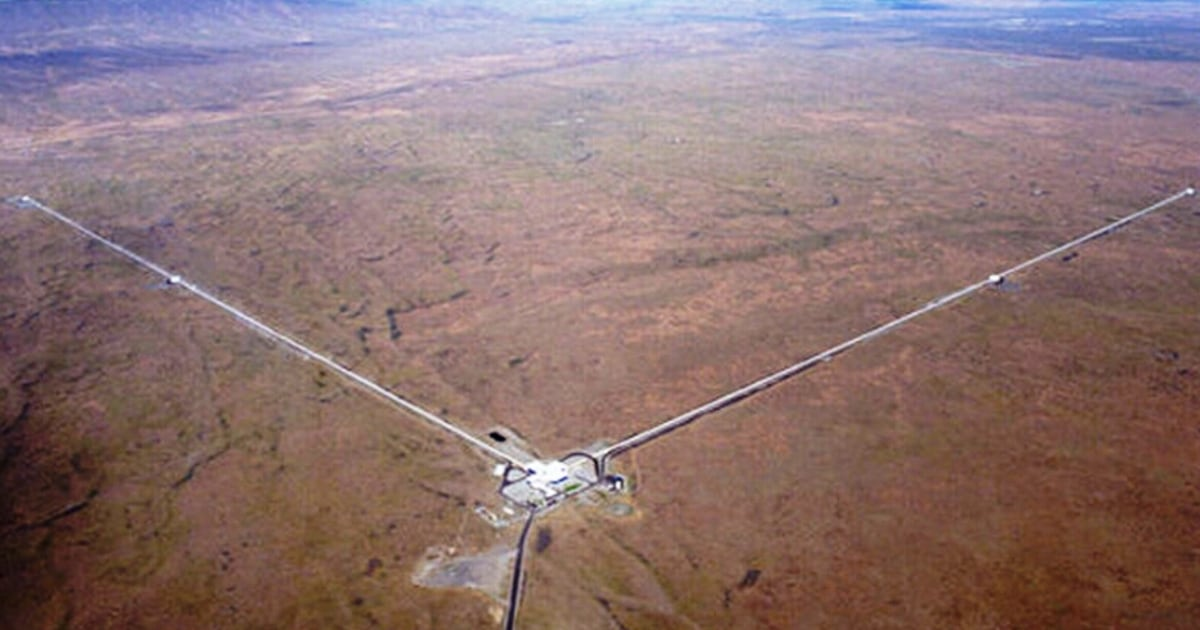
\includegraphics[width=0.6\textwidth]{Images/ligo.jpg}
    \caption{The Laser Interferometer Gravitational-Wave Observatory, or LIGO.}
    \label{fig:ligo}
\end{figure}

At the start of this lab, I said that observational astronomy was ``the art of collecting light.'' This is 95\% true. Let's take a little time to explore that other 5\%; \textbf{Record your responses in your lab write-up}. 
\begin{enumerate}
    %\setcounter{enumi}{17}
    \item Read a little about \textbf{dark matter} at \url{https://www.space.com/20930-dark-matter.html} or \url{https://www.darkmatterday.com/educational-resources-dark-matter-day/}. In which region of the electromagnetic spectrum does dark matter radiate? Why does it make sense to describe dark matter as ``dark''? Can we detect dark matter using any of the telescopes we've looked at in this Lab? What percentage of all the matter in the Universe is attributed to dark matter? Does this number surprise you? The study of dark matter is an extremely rich topic of research in modern astronomy, so stay tuned for further discussion of dark matter in later labs. 
    
    \item When a charged particle is jiggled around, it produces an electromagnetic wave -- that is, a jiggling charged particle produces radiation (which we've looked at extensively in this lab). It turns out that this applies to all matter: when a chunk of matter is jiggled around, it produces \textbf{gravitational waves}, or \emph{gravitational radiation}. Read a little about gravitational waves and the gravitational wave ``telescope'' LIGO (Figure \ref{fig:ligo}) at \url{https://www.ligo.caltech.edu/page/gravitational-waves} and \url{https://www.ligo.caltech.edu/page/what-is-ligo}. What types of objects produce detectable gravitational waves? What astrophysical information can we get from gravitational waves that we can't get from electromagnetic waves? How does LIGO differ from an ordinary light telescope?  
    
    \item \textbf{Neutrinos} are very \emph{very} tiny particles that move at speeds close to the speed of light. Read a little about the neutrino observatory \emph{IceCube} at \url{https://icecube.wisc.edu/about-us/faq/}, at \url{https://icecube.wisc.edu/about-us/facts/}, or at \url{https://icecube.wisc.edu/science/research/}. Where is IceCube located, and why? What astrophysical information can we get from neutrino detections that we can't get from light observations?
    
\end{enumerate}

%%%%%%%%%%%%%%%%%%%%%%% CONCLUSIONS %%%%%%%%%%%%%%%%%%%%%%%
\section{Conclusions}

Complete this section by yourself. \textbf{Record your responses in your lab write-up}.
\begin{enumerate}
    %\setcounter{enumi}{20}
    \item Provide a qualitative description of the electromagnetic spectrum. How does the wavelength of light tie into the electromagnetic spectrum?
    
    \item Briefly explain the importance of observing the Universe in multiple wavelengths. 
    
    \item Why do we need so many different telescopes? Why do we need both space telescopes and ground telescopes?
    
    \item With the coming decades promising rapid advancements in telescopes, detectors, and observatories of all types, the pursuit of \textbf{``multi-messenger''} astronomy -- the combination of observations from electromagnetic radiation, gravitational waves, neutrinos, and cosmic rays to achieve a common scientific goal -- is quickly reaching maturity. Based on what we've covered in this lab, why do you think multi-messenger astronomy is important? What discoveries will we be able to make with multi-messenger observations that we couldn't have made with just observations of light?  
    
    \item Write down at least one question that you still have after finishing this lab.
    
\end{enumerate}

\end{document}
